\documentclass[tikz,border=8pt]{standalone}
% Shared look for every TikZ diagram. Load with \input{../../tools/tikz-style.tex}
\usepackage[T1]{fontenc}
\usepackage{lmodern}
\renewcommand{\sfdefault}{lmr}  % diagrams use the same serif as the text
\usetikzlibrary{arrows.meta, positioning, shapes.geometric, calc, fit, backgrounds}
\definecolor{cblue}{HTML}{4C78A8}
\definecolor{corange}{HTML}{F58518}
\definecolor{cgreen}{HTML}{54A24B}
\definecolor{cred}{HTML}{E45756}
\definecolor{cpurple}{HTML}{B279A2}
\definecolor{cgrey}{HTML}{6B6B6B}
\tikzset{
  every picture/.style={font=\sffamily, line width=1.2pt},
  box/.style={draw=#1, fill=#1!12, rounded corners=4pt, align=center, inner sep=7pt, minimum height=1.1cm},
  box/.default=cgrey,
  arrow/.style={-{Stealth[length=3mm]}, draw=cgrey, line width=1.4pt},
  title/.style={font=\sffamily\bfseries\Large},
  note/.style={font=\sffamily\small, text=cgrey, align=center},
}
\AtBeginDocument{\hyphenpenalty=10000 \exhyphenpenalty=10000}

\begin{document}
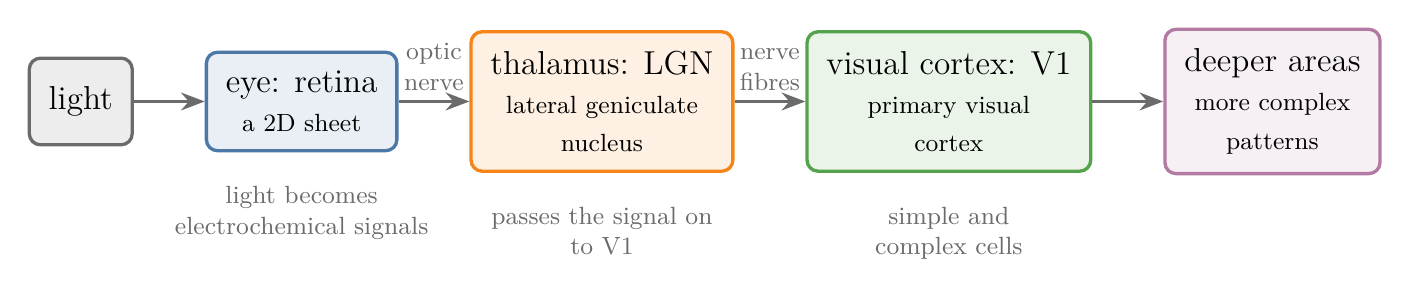
\begin{tikzpicture}[node distance=0.9cm, every node/.append style={font=\sffamily\large}]
  \node[box=cgrey] (light) {light};
  \node[box=cblue, right=of light] (ret) {eye: retina\\\small a 2D sheet};
  \node[box=corange, right=of ret] (lgn) {thalamus: LGN\\\small lateral geniculate\\\small nucleus};
  \node[box=cgreen, right=of lgn] (v1) {visual cortex: V1\\\small primary visual\\\small cortex};
  \node[box=cpurple, right=of v1] (deep) {deeper areas\\\small more complex\\\small patterns};
  \draw[arrow] (light) -- (ret);
  \draw[arrow] (ret) -- node[above, note] {optic\\nerve} (lgn);
  \draw[arrow] (lgn) -- node[above, note] {nerve\\fibres} (v1);
  \draw[arrow] (v1) -- (deep);
  \node[note, below=0.3cm of ret] {light becomes\\electrochemical signals};
  \node[note, below=0.3cm of lgn] {passes the signal on\\to V1};
  \node[note, below=0.3cm of v1] {simple and\\complex cells};
\end{tikzpicture}
\end{document}
